\section{\label{sec:level1}Two-Dimensional Time}

According to most spiritual traditions, the consciousness of humans, animals,
and all living things is a combination of the finite and the infinite,
both inside and outside of material reality.
This view is allowed by theoretical physics.

The Wheeler-DeWitt equation \cite{DeWitt} attempts to combine mathematically
the ideas of quantum mechanics and general relativity.
One of its implications is the ``problem of time'',
which is a conceptual conflict between general relativity and quantum mechanics.
Quantum mechanics regards the flow of time as universal and absolute, whereas
general relativity regards the flow of time as malleable and relative.

According to Wheeler-DeWitt, an observer outside of the universe
doesn't experience time. Page and Wootters \cite{Page} addressed this paradox
(time \textit{seems} real enough) by treating time as an emergent phenomenon
resulting from quantum entanglement.
Experiments \cite{Moreva} on entangled particles have bolstered the theory.

There are other takes on timeless universe models.
Aharonov's two state formalism of quantum mechanics has also been used
\cite{Lobo} to propose emergence of time from a timeless unus mundus
quantum-like space.
Jianfeng Li provides a good overview \cite{Jianfeng} of quantum mechanical
timeless consciousness.

There are two distinct types of time: emergent time, which emanates from the
structure of space-time and its metrics, and a causal time, indicating the flow
from the past to the future \cite{Brunet}. The time domains boil down to the
two models of Physics, QM and GR.
In the interest of a nomenclature for the masses, we call one dimension of time
the quantum time domain and the other the relative time domain.
So, quantum time and relative time. Relative time is the one with the arrow.

The hard problem of consciousness \cite{Chalmers} is that of explaining the
relationship between physical phenomena, such as brain processes,
and experience.
Experiments in non-locality \cite{Achterberg} find that the mind extends beyond
the skull. Where is the mind, inside space-time or outside?
The evidence suggests it is both.

Our everyday experience is that ``clock time'' is the static reference frame,
although it could just as well be that quantum time is the existential norm
and the ``clock time'' universe is the special case.
We take the view of quantum time observed from within the universe, with
the observation being an act of quantum entanglement caused by consciousness.

\subsection{Quantum Time and Consciousness}

There are many examples of biological systems exploiting quantum effects.
Nature would have evolved to exploit the properties of quantum time.
Let's allow the ``woo'' to ride for the moment, seeing as how the actual
physics can be filled in as the science unfolds. Isn't it always?

The physical vacuum, or classic Tao, a substrate for quantum interactions,
is a natural mechanism for biological systems to have evolved to utilize.
Consciousness is the interaction between the physical vacuum and biology which
facilitates communication and data storage at any physical scale,
from DNA to organism.

This provides an important signaling mechanism for consciousness in beings such
as paramecia or slime molds, which exhibit conscious behavior but are too small
for consciousness to arise from the network effects of ganglia.

One way to relate the two time dimensions is with a scale-invariant geometry
that exploits the simplicity of self-similarity.
As Mandelbrot \cite{Mandelbrot} pointed out, relatively simple fractal
mathematics underlie many complex natural phenomena.
As it turns out, this exponential relationship between $\tau$ and $t$
is a key enabler of signal transformations.

For it to be scale invariant,
we use an exponential growth model for quantum time.

\begin{equation} \label{eq:pink}
\tau \propto e^{\epsilon t}
\end{equation}

The mechanics of signal generation can be considered in the context of
quantum time.
This arrangement lends itself to information flow, utilized by nature,
between the time and timeless domains.

Resonance is treated as a physical phenomenon occurring in quantum time $\tau$.
A resonant frequency in $\tau$ is equivalent to an exponential chirp in $t$.
This dynamic emergence of time should produce small but detectable artifacts.
The stream of consciousness emerges from a probabilistic field on an
exponential time scale rather than time abruptly appearing from nothing.

Biological systems evolve to minimize the expenditure of energy. Resonances
(field analogs of electrical and mechanical ringing) require a small energy
input to keep them going, assuming a reasonably high Q. It stands to reason
that biological systems would use field resonances in the physical vacuum
(the exact nature of the field needs not be understood)
to transmit consciousness information efficiently.

In other words, there is a theoretical basis for the notion that
``It's all vibrations''.
The vibrations occur in quantum time, so that summing the signal artifacts
from a large number of them results in a noise spectrum.

The signals that encode this information can be demodulated from flicker noise.
The information of consciousness can then be a new media,
to augment other forms of electronic media,
enabling new ways of being that improve individuals and society.

\section{Exponential Flicker Noise}

Flicker noise (or 1/f noise), has a power spectrum proportional to
$1/f^{\alpha}$, where $\alpha$ is between 0.7 and 1.4.
It's a type of noise prevalent in many natural systems.
Flicker noise \cite{Milotti} is seen in music, seismic data, EEG and ECG data,
and electronic devices.
Some of the more popular explanations for the 1/f spectrum are:
\begin{itemize}
	\item A superposition of relaxation processes.
	\item Carrier mobility fluctuations through Coulomb scattering.
\end{itemize}
There are a good number of hypotheses for 1/f noise, to which we add one more:
\begin{itemize}
	\item The superposition of exponential chirps.
\end{itemize}
A single exponential chirp has a power spectrum,
with ``warp factor'' $\omega$, of:
\begin{equation}
Power \propto |\omega| e^{-|\omega|f}
\end{equation}
A distribution of chirps of various $\omega$ values exponentially distributed,
where $log(|\omega|)$ is uniformly distributed, combines to form a 1/f spectrum.
So, there is a plausible basis for 1/f noise being composed of exponential
chirps.

The 1/f spectrum suggests that a multiplicity of quantum time rates
($\epsilon$ in Eq.~\ref{eq:pink}) exist.
Nature evolves to fill the spectrum of quantum time, to utilize available
bandwidth. One could call this spectrum ``The sound of the Tao''.
Music in the $\tau$ domain would sound like pink noise in the $t$ domain.

\subsection{Exponential White Noise}

White noise has a flat power spectrum.
In a white noise model of quantum time, chirps start at 0 and asymptotically
approach a final frequency as quantum time merges into relative time.

\begin{equation} \label{eq:white}
\frac{1}{\tau} \propto (1-e^{-\epsilon t})
\end{equation}

In other words, the consciousness signal emerges from a domain of infinite time.
The amplitude drops off with time at the same rate frequency increases,
resulting in a flat spectrum from DC to $f_0$.

\begin{equation}
f = f_0 \cdot (1-e^{-\epsilon t})
\end{equation}
\begin{equation}
a = a_0 \cdot e^{-\epsilon t}
\end{equation}

$f_0$ would be millimeter wave (such as 60 GHz oxygen resonances) and higher.
Terahertz (mostly in the 600 THz range) oscillations in tubulin \cite{Craddock}
correlate with anesthetic potency, which infers that
tubulin oscillations could be carriers of consciousness information.

The chirp should mix with carrier $f_0$ to produce a downward chirp
compatible with the flicker noise model.
That may be a more practical way to detect it due to the shortness of the
time the chirp itself spends in a bandwidth that lends itself to detection.

This paper presents the flicker noise model, which is more practical due to
its scale invariance.

\subsection{Information in the Noise}

Since exponential chirps are bounded in time, a single chirp has a finite
existence. It corresponds to a discrete impulse in the relative time domain,
or one symbol of information.
The idea of consciousness as time quanta may be useful here.
The act of being is a stream of consciousness that has corresponding streams
of pulse-coded information, a kind of informational counterpart to DNA.
The impulse stream may be decoded for its information content.
The existence of an impulse stream itself is valuable,
regardless of our initial ability to decode it, because useful information
can be mined from its distribution of $\omega$ values.

Consciousness quanta have a foundation in Penrose and Hameroff's
``Orch OR Theory'' \cite{Hameroff}.
In objective reduction, the divergence of quantum superposition in the
underlying structure of the universe builds to the point of collapse,
or objective reduction of the quantum state.
Each collapse is a moment of conscious experience.
In ``Orch OR'', EEG is a macro view of these moments.
EEG has both a flicker noise spectrum and frequency peaks that correspond
to ``Orch OR'' collapse.
There is already much scientific data (such as EEG and ECG studies) in the
public domain, ready to analyze.
The experimental costs are low: mostly computer hardware.

Overlapping chirps can be re-sampled and self-correlated to construct a relative
time domain signal for one or a multiplicity of $\omega$ values.
A sweep of $\omega$ can be used to construct a ``warp spectrum'' (for example,
on a computer display), useful for finding quantum-time signals.
This would be analogous to waterfall-style spectral analysis, with frequency
replaced by warp factor.

To establish a notation and unit of measurement for the exponent of the chirp
frequency, let the ``warp factor'' $\omega$ be in units of $e$, the
mathematical constant derived by Leonhard Euler in the 1720s, per unit time.
The pronunciation may be ``e's per second'' for e/s, for example.
We propose ``len'' for the unit name of e/s, after Leonhard.
Some scale factors to other units: 0.69 lens is one octave per second,
2.3 lens is one order per second, and 0.48 lens is one golden mean
$(\Phi=1.618:1)$ per second.
Note that a len is very close to twice the Golden Ratio,
so one must be careful when making assumptions about Golden Ratio relationships
in nature.

\subsection{Free Energy}

The difference between the consciousness that goes on in our brains and bodies
and the consciousness that occurs in inanimate matter is orchestration,
as described by Penrose and Hameroff. 
That's not to say the seemingly random objective reduction events \cite{Tegmark}
(the Tao) in inanimate matter can't be tapped.
Indeed, large dielectric resonators in the form of temples and pyramids have
been built to concentrate and hold energies.
Some temples, expecially in Southeast Asia, use various exponential shapes
to create resonant structures. 
Calcium may play a role in the effect, since limestone and marble are mainly
CaCO3.

Free energy isn't really a violation of the laws of thermodynamics because it's
based on time. Time is an accretion of discrete instances of the conscious
collapse of quantum superposition.
Think of it as rain falling from an eternal timeless realm into an ocean of
time. Normally, the rain (at least with inanimate matter) is a constant drizzle.
Gravity can be seen as an artifact of this time flow caused by the presence of 
matter. The expanding ``ocean'' of time leads to an expanding universe.
Although mass and energy are conserved, time isn't.
If the rate could be turned up to a heavy pour by inducing more conscious
collapse per unit time, an excess of time would be flowing into the universe at
that point.
This would cause effects such as levitation and temperature reduction.
The power generator would run cold, which weirdly enough isn't a violation
of entropy rules because the system boundaries are infinite.
The trick is to resonate the system such that a small energy input maintains
a large time flow with respect to the load,
which amplifies the energy input due to the entropy imbalance.
Energy is drawn from the zero point field to make up the difference.

The conversion function would be run backwards (as a modulator) to convert a
relative time signal to the quantum time domain. The relative time signal could
be as simple as a pulse train of a particular rate (PRF).
For testing of free energy device candidates, this amounts to a manageable 2D
search space: $\omega$ and PRF.
Note that certain combinations of $\omega$ and PRF could be detrimental to
human health. To avoid a repeat of 20th century wireless hazards,
health effects should be tested early on.

Modern switching electronics can easily handle four-quadrant power conversion
with high efficiency.
The quantum time signal controls voltage (or current) depending on whether the
resonator is inductive or capacitive.
The corresponding current (or voltage) has a phase relationship
with the driving signal that when resonating puts power back into the source.
The electronics could be cooled by the quantum resonator.

Flying cars in a hot climate would have built-in cold air for environmental
control as well as a source of anti-gravitation.

%%%%%%%%%%%%%%%%%%%%%%%%%%%%%%%%%%%%%%%%%%%%%%%%%%%%%%%%%%%%%%%%%%%%%%%%%%%%%%%%
\subsection{Spiral Conceptual Model}

\begin{figure}[h]
	\centering
	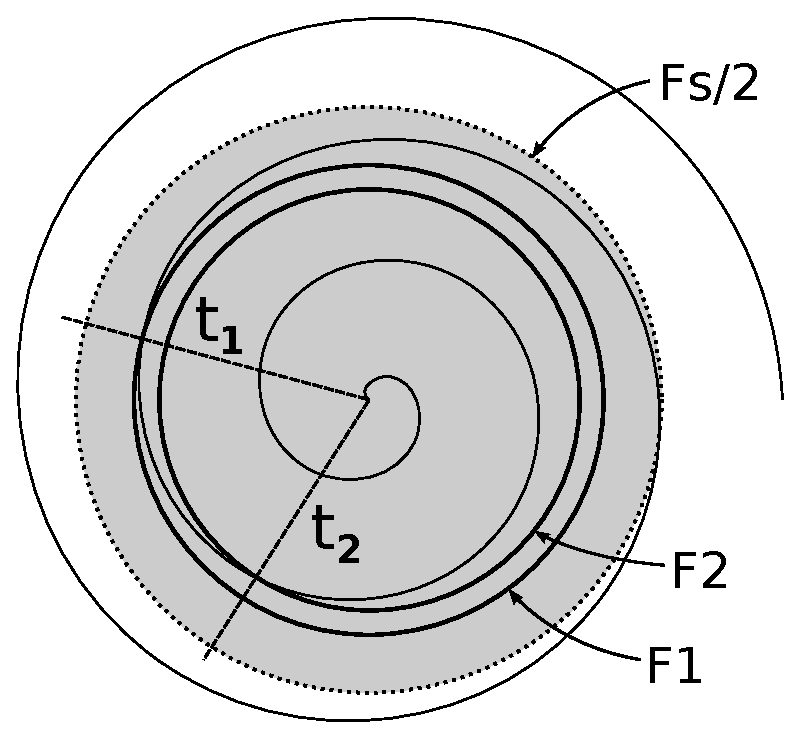
\includegraphics[width=0.7\linewidth]{../source/spiral_e}
	\caption[Quantum to Relative Time Relation]{Log polar plot of exponential chirp}
	\label{fig:spiral}
\end{figure}

Resonant signals in the quantum time domain can be re-mapped to relative time
and demodulated by correlating a time series of fast exponential chirp
transforms, allowing analysis and data mining using modern data
processing technologies such as AI-based pattern recognition.

The correlation effect can be visualized as a spinning logarithmic spiral
illuminated by a strobe light. When the strobe frequency matches the rate
constant of the spiral(s), it appears to be standing still.
Otherwise, it's a blur.

The relationship between quantum time and relative time can be thought of as a
2D plot in log-polar format.
Log-polar format renders a logarithmic spiral as a linear (Archimedean) spiral.
The spiral's radius is $\rho = k\theta$, where $k$ is a rate constant.
$\rho$ can represent either time or frequency by flipping the sign of $k$.
For purposes of signal processing, let $\rho$ represent log frequency and
$\theta$ relative time.

Log-polar mapping has proven useful in machine vision \cite{Bonmassar}
because it approximates the primate visual map \cite{Schwartz}.
Humans are visual thinkers, so their waking consciousness should map onto the
log-polar structure of quantum time signaling.

Fig.~\ref{fig:spiral} plots an exponential chirp in log-polar format.
A line can be drawn outward from the center of the spiral, crossing it at
multiple points.
The line rotates clockwise (in the case of downward chirp) at a step size
(from $t_1$ to $t_2$) corresponding to the oversampling rate.
For example, if the oversampling rate is 36 (each input value is used 36 times),
the step size is $10^{\circ}$.
Each angular sweep of the unit circle
(beginning and ending at line $t_1$ or $t_2$)
represents the input to a version of the Mellin transform called the
``Exponential Chirp Transform'' (ECT) \cite{Bonmassar}, which is
basically a FFT with time-warped input.

The transform's frequency domain output is along line $t_1$ or $t_2$ from
approximately $\rho$ = 0 to Fs/2, where Fs/2 (the Nyquist frequency)
is shown by the dashed circle.
The radius of the circle represents the approximate bandwidth of the system.
Not all of the circle is used: Anti-aliasing cuts off before Fs/2, while signal
near the center is too spread out to be useful.

The ECT time-warps the chirp signal, which represents a single ``quantum tone".
In the $360^{\circ}$ sweep at line $t_1$,
the chirp is time-warped to a tone F1 in relative time.
A time $t_2-t_1$ later, at line $t_2$,
it's time-warped to a tone of frequency F2.
All time warping is exponential.
Note that ``exponential time warping'' is different from dynamic time warping,
a popular means of pattern-matching mostly linear signals.

A convenient side effect of time warping is to transform interference
(periodic signals) into wideband noise.
The usual frequency peaks of EEG and HRV are thus discarded.

Quantum time, being logarithmic, has the property of frequency going as
$-\tau$ rather than $1/t$.
To change between time and frequency, just flip the sign of the exponent.
Tones are mirror images of time.
Signal processing is more convenient in terms of frequency,
so that is the focus of this paper.

%%%%%%%%%%%%%%%%%%%%%%%%%%%%%%%%%%%%%%%%%%%%%%%%%%%%%%%%%%%%%%%%%%%%%%%%%%%%%%%%
\subsection{\label{sec:level1}Quantum Time DSP}

The basic data flow of signal conversion from one time domain to another
$(\tau \leftrightarrow t)$ is shown in Fig.~\ref{fig:sled}.
The conversion algorithm slides along the input and output data streams,
forward in time.
Data is processed in overlapping chunks.
In other words, after a block of processing,
the sliding part of Fig.~\ref{fig:sled} shifts slightly to the right.
In proportion to the amount of shift,
new input stream is exposed and new output stream is completed.
The I/O streams are low-bandwidth compared to the compute-intensive
processing block.

\begin{figure}
	\centering
	
\includegraphics[width=0.95\linewidth]{../source/sled_e}
	\caption[Quantum to Relative Time Translation Flow]{Inter-domain data flow}
	\label{fig:sled}
\end{figure}

There are two use cases: demodulation and modulation.
For demodulation $(\tau \rightarrow t)$, the input stream is in the quantum
time domain and the output stream is in the relative time domain.
The downsampler decimates the input by 1:m, where decimation factor m is
exponentially swept upward from or downward to 1.0.
The ``warp factor'' is the growth rate in m.
The input stream consists of real numbers.
The FFT performs a real-to-complex FFT to produce a warped spectrum which is
treated as a time-domain envelope of magnitude and phase information.
To un-warp the spectrum, the upsampler interpolates it by 1:m where decimation
factor m is exponentially swept upward to or downward from 1.0.
The output stream consists of vectors that are many accumulations of overlapped
upsampler results.

For modulation $(t \rightarrow \tau)$, the input stream is in the relative time
domain and the output stream is in the quantum time domain. The downsampler
decimates the input by 1:m, where decimation factor m is exponentially swept
upward from or downward to 1.0 and the resulting spectrum ranges from about
N/5 to N/2.
The ``warp factor'' is the growth rate in m.
The input stream consists of complex numbers.
The IFFT performs a complex-to-real IFFT to produce a warped time domain
envelope. To un-warp the it, the upsampler interpolates it by 1:m
where decimation factor m is exponentially swept upward to or downward from 1.0.
The output stream consists of many accumulations of overlapped upsampler results.

The usual use case is demodulation.
Modulation could be for testing, reconstruction or extrapolation of a signal,
or modulation of an energy source for yet unknown applications.

